\documentclass[10pt]{beamer}
\usetheme[progressbar=frametitle,subsectionpage=progressbar]{metropolis}
\usepackage{appendixnumberbeamer}
\usepackage{booktabs}
\usepackage{makecell}
\usepackage{multicol}
\usepackage{xspace}
\usepackage{emoji}
\usepackage{tabularx}
\usepackage[autolanguage]{numprint}
\usepackage[backend=biber,style=authortitle,maxcitenames=1]{biblatex}

\usepackage{pgfpages}

%\setbeameroption{show notes on second screen}

\addbibresource{references.bib}
\ExecuteBibliographyOptions{isbn=false,url=false,doi=true,eprint=false}
\DeclareSourcemap{
  \maps[datatype=bibtex, overwrite]{
    \map{
      \step[fieldset=editor, null]
      \step[fieldset=booktitle, null]
      \step[fieldset=series, null]
      \step[fieldset=pages, null]
      \step[fieldset=address, null]
      \step[fieldset=journal, null]
      \step[fieldset=publisher, null]
      \step[fieldset=volume, null]
      \step[fieldset=number, null]
      \step[fieldset=note, null]
    }
  }
}

% Simpler references
\def\do#1{
  \DeclareBibliographyDriver{#1}{%
    \usebibmacro{bibindex}%
    \usebibmacro{begentry}%
    \usebibmacro{author/editor+others/translator+others}%
    \setunit{\labelnamepunct}\newblock
    \usebibmacro{title}%
    \newunit\newblock
    \usebibmacro{date}%
    \newunit\newblock
    \iftoggle{bbx:doi}
      {\printfield{doi}}
      {}%
    \setunit{\bibpagerefpunct}\newblock
    \usebibmacro{pageref}%
    \newunit\newblock
    \usebibmacro{finentry}}}
\makeatother

% Breadcrumbs
\setbeamertemplate{mini frame}{}
\setbeamertemplate{mini frame in current section}{}
\setbeamertemplate{mini frame in current subsection}{}

\makeatletter
\setbeamertemplate{footline}{%
  \begin{beamercolorbox}[wd=\textwidth, sep=2ex]{footline}%
    \usebeamerfont{page number in head/foot}%
    \usebeamertemplate*{frame footer}
    \hfill%
    \usebeamertemplate*{frame numbering}\vskip-2pt
  \end{beamercolorbox}%

  \begin{beamercolorbox}[colsep=1.5pt]{upper separation line head}
  \end{beamercolorbox}
  \begin{beamercolorbox}{section in head/foot}
    \vskip2pt\insertnavigation{\paperwidth}\vskip-2pt
  \end{beamercolorbox}%
  \begin{beamercolorbox}[colsep=1.5pt]{lower separation line head}
  \end{beamercolorbox}
}
\makeatother
\setbeamercolor{section in head/foot}{fg=normal text.bg, bg=lightgray}

\newcommand{\PresQ}[0]{\textsc{PresQ}\xspace}
\newcommand{\eqdist}{\stackrel{d}{=}}

% Only sections on the index
\setcounter{tocdepth}{1}

% 2. El acto consistirá en la exposición oral por el doctorando del trabajo de
% investigación elaborado ante los miembros del tribunal, refiriéndose
% principalmente a la labor realizada, la metodología, el contenido y las conclusiones,
% haciendo especial mención de sus aportaciones originales.

% Evaluación
% i. Justificación del carácter innovador del tema de estudio.
% ii. Adecuación de la metodología utilizada o propuesta de alternativas
% iii. Grado de claridad en la exposición de los resultados obtenidos y análisis de los mismos.
% iv. Observación de la correcta elección y citación de la bibliografía.
% v. Análisis crítico de las conclusiones de estudio.


\title{Navigating Diverse Datasets\\
in the Face of Uncertainty}
\subtitle{}
\date{September 11, 2023}
\author{Alejandro Álvarez Ayllón}
\institute{
Tesis dirigida por Dr. Juan Manuel Dodero Beardo y Dr. Manuel Palomo Duarte \\
Programa Oficial de Doctorado en Ingeniería Informática de la Universidad de Cádiz
}
\titlegraphic{\hfill
\includegraphics[height=1.5cm]{uca-logo.pdf}}

\begin{document}

\maketitle

\begin{frame}{Overview}
\tableofcontents
\end{frame}

\section{Introduction}

\begin{frame}{Motivation}
\begin{enumerate}
    \item Data exploration represents the fourth paradigm of scientific exploration, alongside experimental, theoretical, and computer-simulation.
    \item Data exploration is a vital component of the data-intensive scientific process.
    \item Researchers must curate, understand, and extract information from data sets.
    \item To extract knowledge, first, they need to identify patterns: \alert{data mining}.
\end{enumerate}
\end{frame}

\begin{frame}{Our Focus: Data Understanding}

\alert{Familiarization with the data}: The user interactively explores the
data, gaining insight, and generating new hypotheses.

During this stage, the data may be stored in unprocessed files with an
inconsistent or poorly documented schema.

\note{
\begin{itemize}
    \item A part of Data Mining is Data Understanding.
    \item As Hector García Morales noted, \emph{most of the attention when developing Machine Learning and AI systems is put in  modeling and training (data preparation). Still, a successful model relies almost entirely on a well-structured database and a properly identified set of features.}
    \item For instance, in Astronomy, there can be catalogs with data from the same part of the sky, done by someone
        with some Python script stored somewhere.
\end{itemize}
}
\end{frame}

\begin{frame}{Objectives}
\begin{alertblock}{Main Objective}
    \smallskip
    To assist data scientists while exploring unprocessed, numerical, raw data distributed across multiple
    files based solely on its intrinsic distribution.
\end{alertblock}

\begin{block}{Sub-objectives}
    \begin{enumerate}
        \item Find existing techniques that help users to explore the data in situ.
        \item Identify gaps in the coverage of the existing techniques.
        \item Design new algorithms tailored to numerical, uncertain data.
    \end{enumerate}
\end{block}

\note{
Focusing on \alert{multidimensional} distributions.
}
\end{frame}

\section{Methodology}

\begin{frame}{Framework}
\begin{block}{\alert{Researching Information Systems and Computing}~\footcite{Oates2006}}

\begin{description}
    \item[Purpose] The stated objective.
    \item[Products] Analysis of the state-of-the-art, and two new algorithms.
    \item[Process] See next slide.
    \item[Participants] Researcher, supervisor, reviewers.
    \item[Paradigm] \emph{Pragmatism}.
    \item[Presentation] Papers, posters, published software, the current dissertation, etc.
\end{description}

\end{block}

\note{
\begin{itemize}
    \item \alert{Paradigm} Shared world view, not provable.
    \item \alert{Pragmatism}, knowledge is approximate and must be evaluated by its utility. 
    \item Other examples would be positivism (reality is objective, research neutral, i.e., physics) and critic research (social structure is the focus).
    \item \alert{Important to evaluate the added knowledge from the thesis}
\end{itemize}
}
\end{frame}

\begin{frame}{Process Model}
\begin{figure}
    \centering
    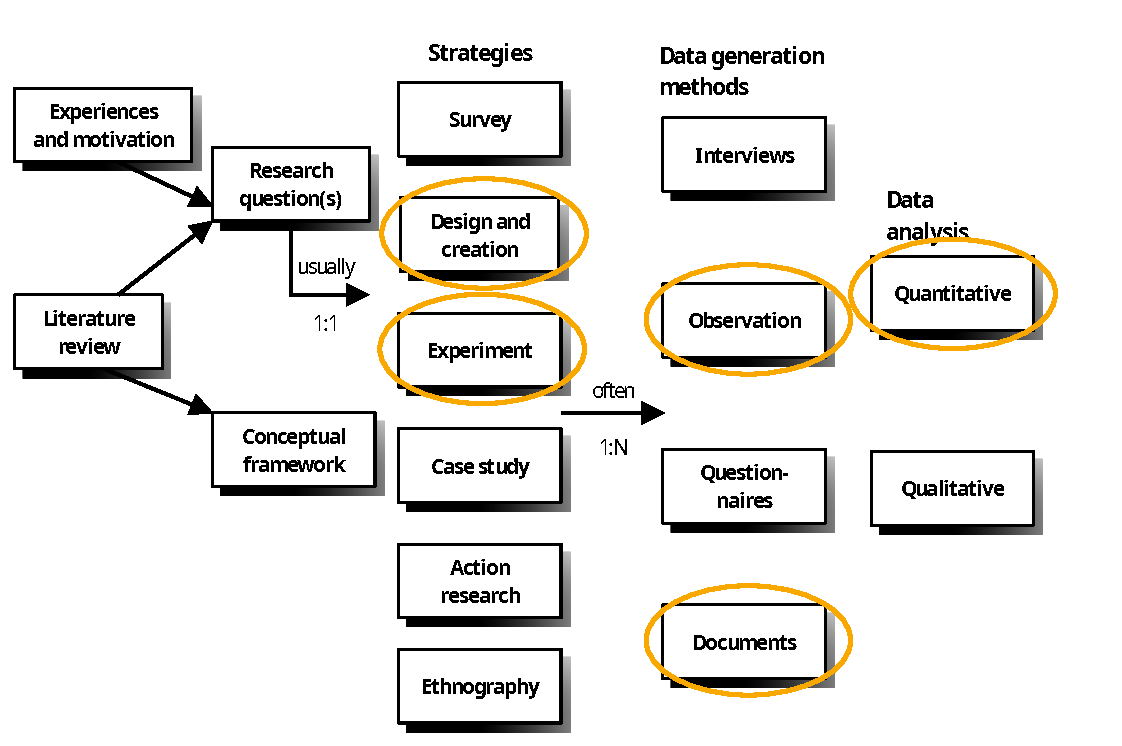
\includegraphics[width=\textwidth]{modelo_proceso_circle.pdf}
\end{figure}

\note{

\begin{alertblock}{Literature Review}
    \smallskip
    \cite{Petersen2007}, a process for exploring
    the situation of a wide research area with a high level of granularity.
\end{alertblock}

\begin{alertblock}{Strategy}
    \smallskip
    \cite{Dym2012}, the systematic, intelligent generation and evaluation
    of specifications for artifacts whose form and function achieve stated objectives and satisfy specified
    constraints.
\end{alertblock}

} % end note

\end{frame}

\section{State of the Art}
\begin{frame}{Systematic Literature Mapping}
\begin{alertblock}{Questions}
    \begin{itemize}
        \item RQ1. How has Interactive Data Exploration research evolved since 2015?
        \item RQ2. What is the maturity level of the research area?
        \item RQ3. How far are we from a tool that provides \alert{interactive} access
            to \alert{raw} data files stored in \alert{distributed} storage?
    \end{itemize}
\end{alertblock}
\begin{block}{Search strategy}
    \begin{itemize}
        \item Backward Snowballing \cite{Idreos2015}
        \item Forward Snowballing
        \item Digital Libraries (ACM, Elsevier, Springer, IEEE, \ldots)
        \item Two searches: 2017 and 2022
    \end{itemize}
\end{block}
\note{
\begin{itemize}
    \item Since 2015 because Idreos 2015 is the bootstrap.
    \item Access at a higher granularity than file (how data is sharded is an "implementation detail")
\end{itemize}
}
\end{frame}

\begin{frame}{Results}
    \begin{table}
    \small
    \begin{tabularx}{\textwidth}{r r r r r r} \hline
    \bf Accepted & \bf Duplicated & \bf Not Primary & \bf Off Topic & \bf Too Old & \bf Total \\ \hline
    \multicolumn{6}{c}{\textbf{2017}} \\
    242 & 9 & 16 & \numprint{5 295} & 126 & \numprint{5 688} \\
    \numprint[\%]{4.25} & \numprint[\%]{0.16} & \numprint[\%]{0.28} & \numprint[\%]{93.09} & \numprint[\%]{2.22} & \numprint[\%]{100} \\
    \\
    \multicolumn{6}{c}{\textbf{2022}} \\
    89 & 1 & 19 & \numprint{2359} & 0 & \numprint{2468} \\
    \numprint[\%]{3.61} & \numprint[\%]{0.04} & \numprint[\%]{0.77} & \numprint[\%]{95.58} & \numprint[\%]{0.00} & \numprint[\%]{100} \\
  \end{tabularx}
  \caption{Accepted and rejected papers count.}\label{tab:mapping/acceptance}
\end{table}
\end{frame}


\begin{frame}{Classification}
\begin{figure}
    \centering
    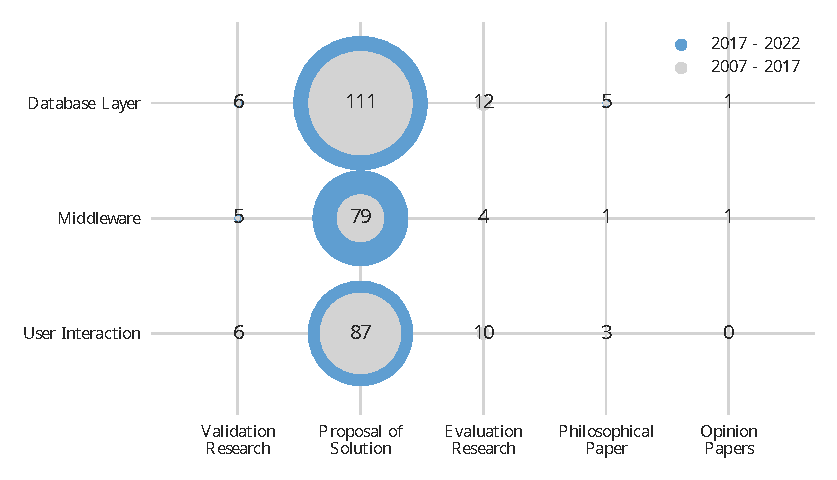
\includegraphics[width=\textwidth]{layer_vs_type.pdf}
    \caption{Layer vs. Study research type.}
\end{figure}
\end{frame}

\begin{frame}{Conclusions}
    \begin{block}{RQ1. How has the research area evolved?}
        \begin{figure}
            \centering
            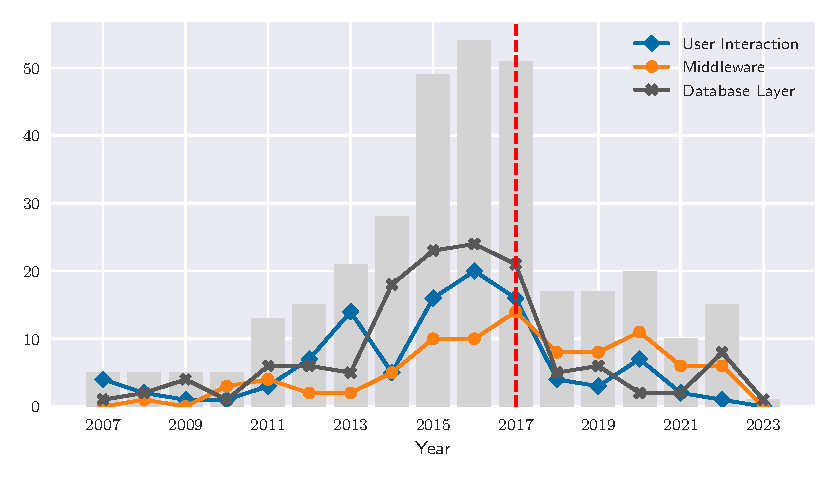
\includegraphics[width=0.8\textwidth]{layer_histogram.pdf}
            \caption{All three layers are well studied, but the middleware layer is becoming a more popular target.}
        \end{figure}
    \end{block}
\end{frame}
        
\begin{frame}{Conclusions}
    \begin{block}{RQ2. What is the maturity level of the research area?}
        \begin{table}
        \begin{tabularx}{\textwidth}{r r r r r} \hline
            \bf Validation & \bf Proposal & \bf Evaluation & \bf Philosophical & \bf Opinion \\ \hline
            17 & 277 & 26 & 9 & 2 \\
            \numprint[\%]{5.14} & \numprint[\%]{83.69} & \numprint[\%]{7.85} & \numprint[\%]{2.72} & \numprint[\%]{0.60}
        \end{tabularx}
        \caption{
            The vast majority of studies are \emph{Proposal of Solutions}. There is very little follow-up of implementations in practice.        
        }
        \end{table}    
    \end{block}
\end{frame}

\begin{frame}{Conclusions}
    \begin{block}{RQ3. How far are we from a tool that solves our three requirements?}
        \begin{figure}
            \centering
            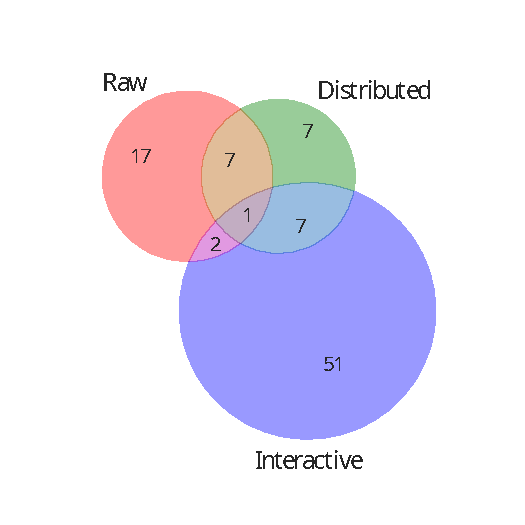
\includegraphics[width=0.4\textwidth]{venn.pdf}
        \end{figure}
        \cite{Han2017}
    \end{block}

\note{
    Not explicitly interactive, but within limits
}
\end{frame}

\begin{frame}{Threats to Validity}
\begin{itemize}
    \item Lack of well-defined keywords
    \item Search bias (i.e., set of online libraries)
    \item Classification bias (researcher's)
\end{itemize}
\end{frame}

\begin{frame}{Insights}
    \begin{block}{}
        Most solutions treat files as independent relations. They offer
        little assistance in finding \textit{overlapping} relations: \alert{Schema Homogenization}.
    \end{block}
    \begin{block}{One exception: \textsc{Kayak}~\footcite{maccioni_crossing_2017}, integrates \textsc{Metanome}~\footcite{papenbrock2015data}}
    \smallskip
    \centering
        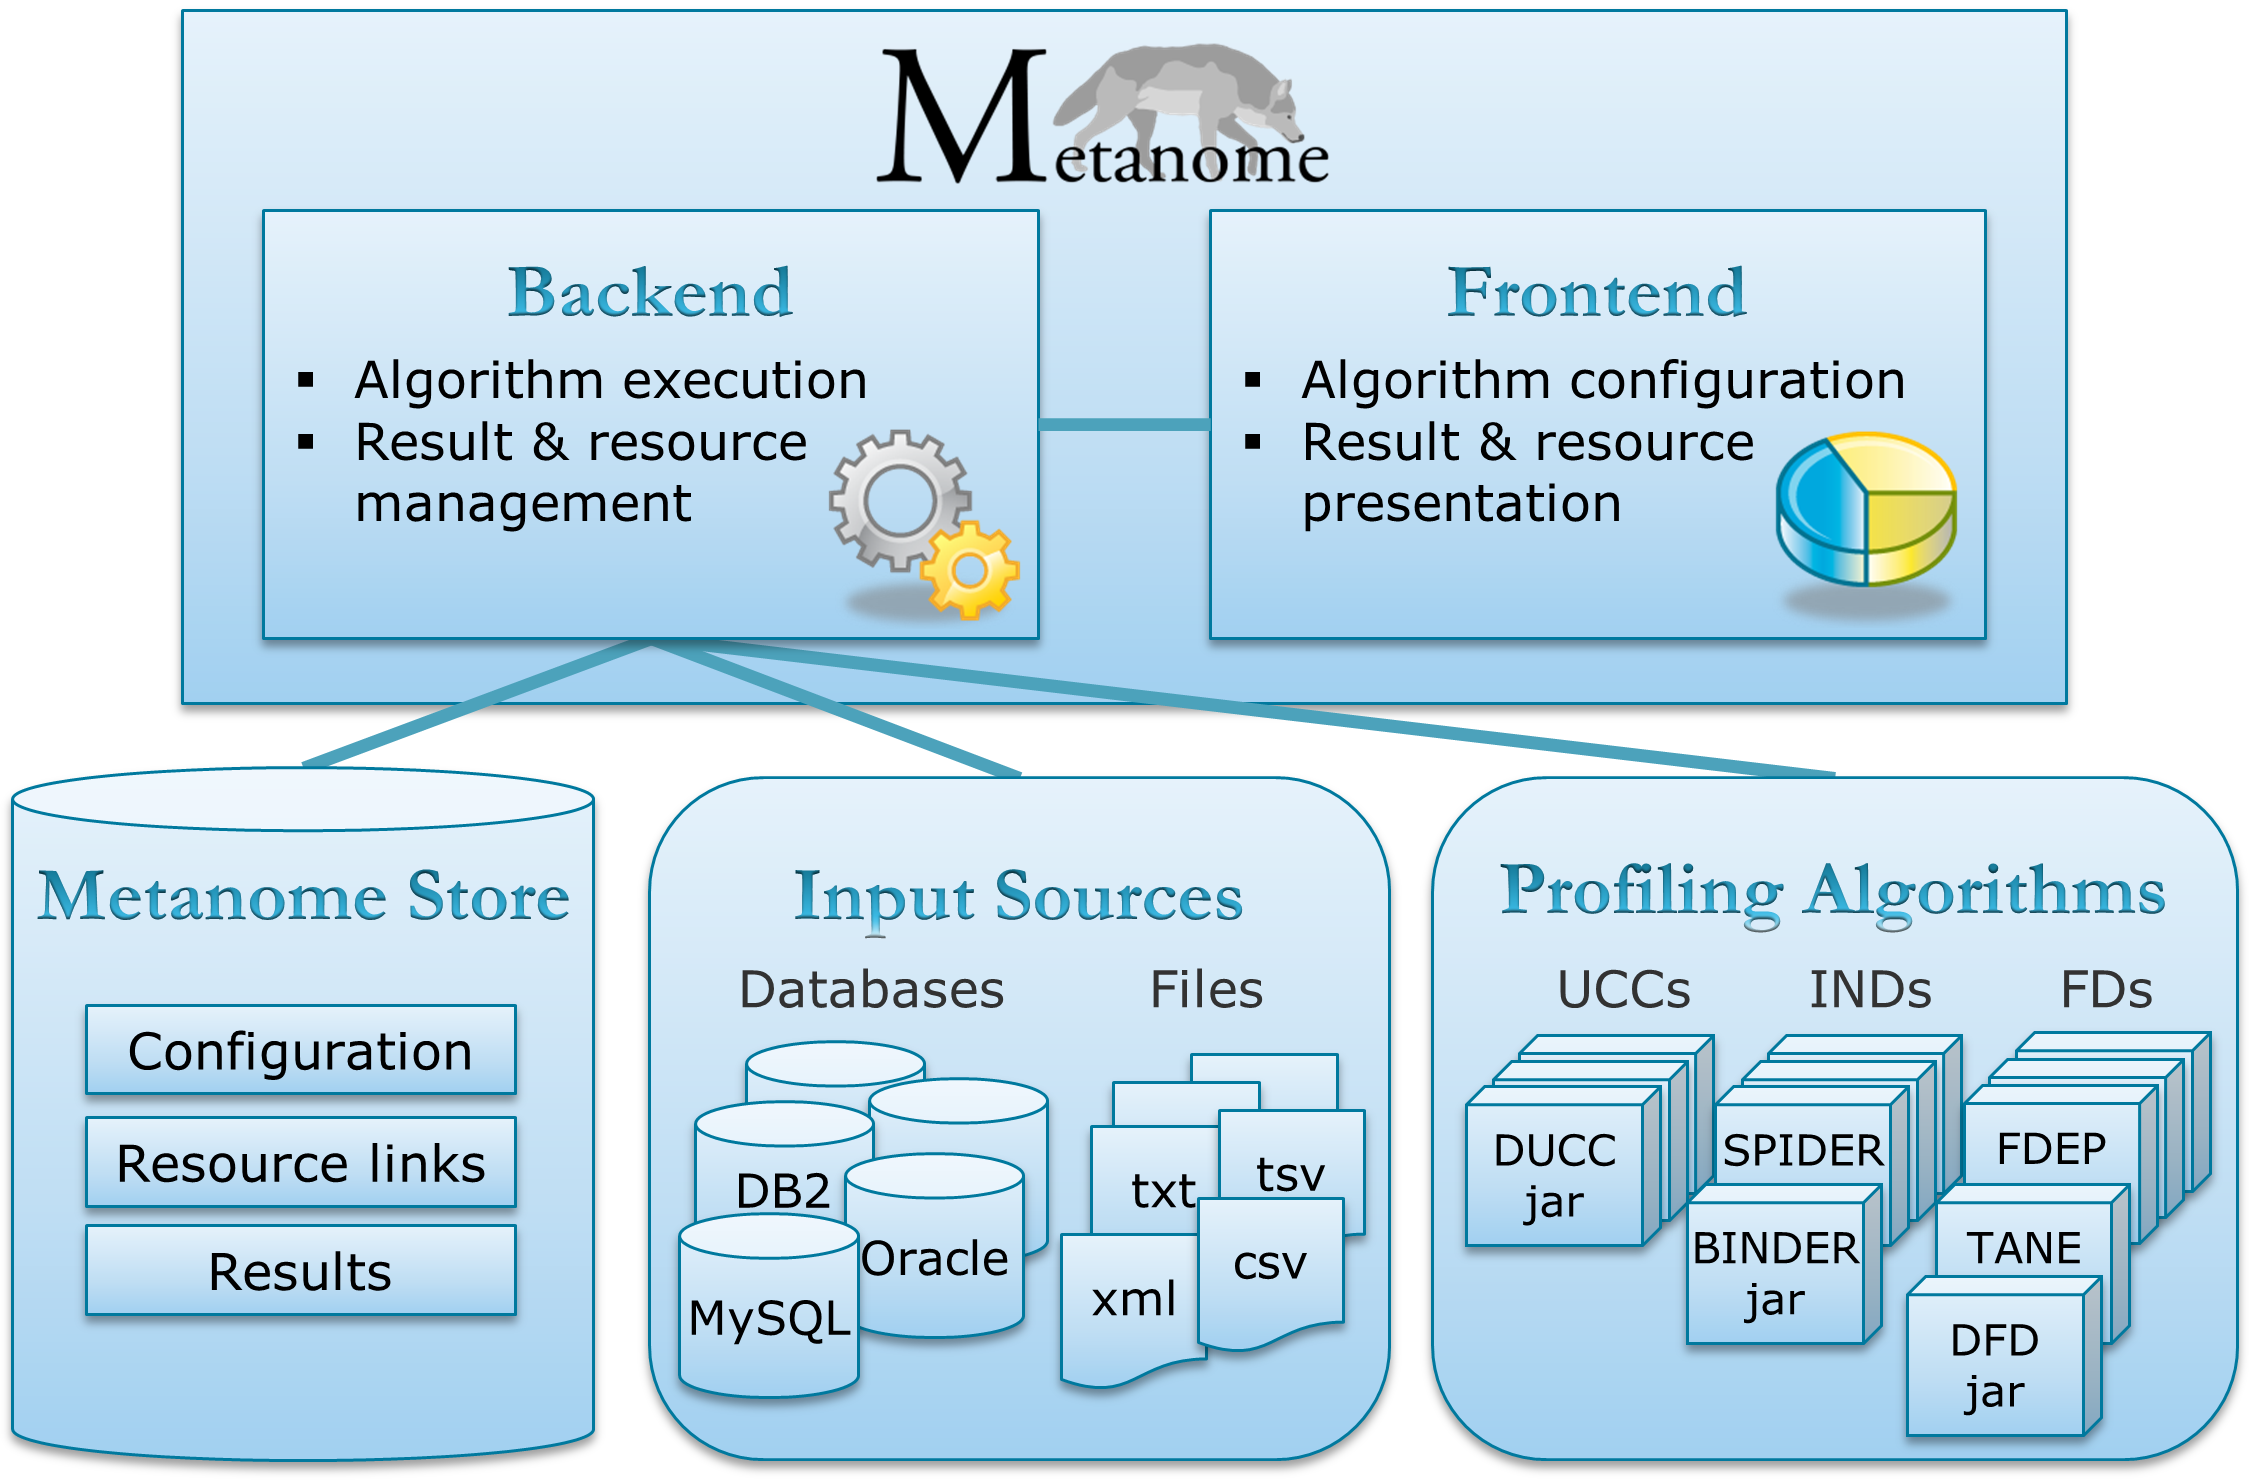
\includegraphics[width=0.5\textwidth]{metanome.png}
    \end{block}

\note{
    Based on \emph{Inclusion Dependencies} (IND): discrete data types.
    
    BACKUP
    \cite{alawini2016} considers numerical attributes, but only 1D.
}
\end{frame}

\begin{frame}{Inclusion Dependency (IND)}
    \begin{block}{}
        \smallskip
        An inclusion dependency between column A of relation
        R and column B of relation S, written $R.A \subseteq S.B$, asserts that each
        value of A appears in B. Similarly, for two sets of columns X
        and Y , we write $R.X \subseteq S.Y$ , or $X \subseteq Y$ , when each distinct
        combination of values in X appears in Y~\footcite{Casanova1984,DeMarchi2002,abedjan2015}
    \end{block}
\note{
How do we go from 1-EDD to 2-EDD to n-EDD? We need to define an order.
}
\end{frame}

\begin{frame}{Definition of the Search Space}
    \metroset{block=fill}    \begin{block}{Inference Rules}
        \begin{itemize}
            \item Reflexivity, Transitivity, Permutation and Projection
        \end{itemize}
    \end{block}
    \begin{block}{Partial Order}
        Let $I_1 = R[X] \subseteq S[Y]$ and $I_2 = R'[X'] \subseteq S'[Y']$.       
        $I_1$ \textbf{specializes} $I_2$ (denoted $I_1 \prec I_2)$ iff
        \begin{enumerate}
            \item $R = R'$ and $S = S'$.
            \item $X$ and $Y$ are sub-sequences of $X'$ and $Y'$, respectively.
        \end{enumerate}
    \end{block}
    \begin{block}{Satisfiability}
         Let $I_1$, $I_2$ be two candidate INDs such that $I_1 \prec I_2$, and $d$ a dataset.
         $d \models I_i$ denotes that an IND $I_i$ exists on the dataset.
         \begin{enumerate}
             \item If $d \models I_2$, then $d \models I_1$
             \item If $d \not\models I_1$, then $d \not\models I_2$
         \end{enumerate}
    \end{block}
\note{
    Partial order, the second point, is possible thanks to the inference rules.
    We can take a subset, shuffle (both sides), and still hold.

    Satisfiability allows purging search space.
}
\end{frame}

\begin{frame}{Search Space}
\begin{figure}
    \centering
    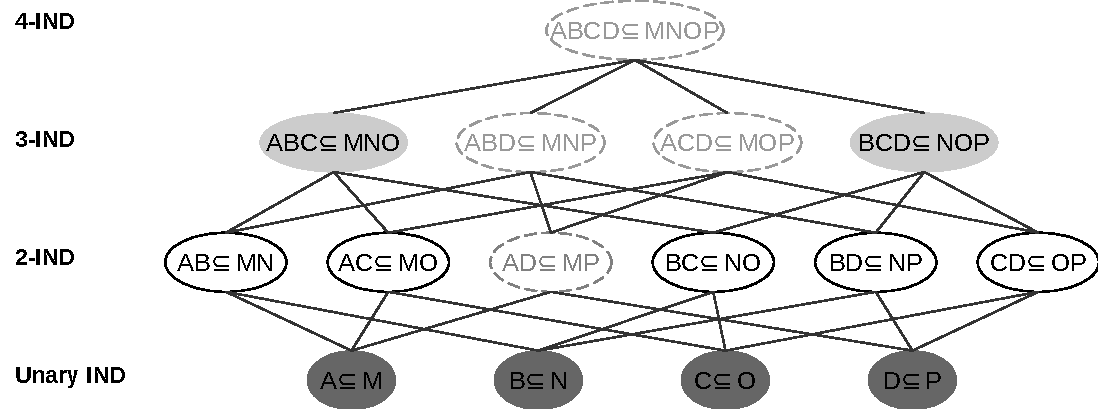
\includegraphics[width=\textwidth]{lattice.pdf}
    \caption{Search space for INDs}
\end{figure}
\note{
    Lattice!
    We can have something like this thanks to specialization (a partial order).
}
\end{frame}

\begin{frame}{Traversal}
    \begin{block}{Naive Traversal of the Search Space}
        \smallskip
        We can validate pairwise INDs. Then, we build possible three-wise INDs and validate them.
        Then, we build possible four-wise INDs...
    \end{block}
        
    \begin{alertblock}{Complexity}
    \smallskip
    Generally, if we have an n-IND between two datasets and traverse the lattice bottom-up,
    the number of possible combinations we need to test is as follows:
    
    \begin{equation*}
        \sum_{k=1}^{n}{\binom{n}{k}} = \sum_{k=1}^{n} \frac{n!}{n!(n - k)!}
    \end{equation*}
    
    \end{alertblock}

    \begin{block}{Top-Down Traversal}
        It works well for high-dimensional INDs but has the same complexity if they are
        low-dimensional.
    \end{block}

\end{frame}

\begin{frame}{Complexity}

    It turns out that finding INDs is one of the hardest computer science
    problems~\footcite{Blsius2017}.
    
    \begin{itemize}
        \item It is \textbf{NP-hard}.
        \item The \textbf{number of solutions} can be \textbf{exponential} in the input size.
        \item It is \textbf{non-approximable} (NP-hard even if we accept an error margin).
        \item However, alternating Bottom-Up and Top-Down works well for
            typical problems.
    \end{itemize}
    
    \bigskip

\note{
\begin{itemize}
    \item BACKUP:

    \item The decision problem of whether there is a clique of a
    certain minimum size in a graph is NP-complete. Thus, finding all
    cliques in a graph is NP-hard\footcite{koeller2002integration}.
    
\end{itemize}
}
\end{frame}

%\subsection{Clique Finding}
\begin{frame}{Clique Finding}
    \textsc{Find2}~\footcite{koeller2003discovery} maps the problem to finding cliques on hypergraphs.
    \begin{description}
        \item[Hypergraph] Generalization of a graph, an edge connects multiple nodes.
        \item[Clique] Subset of nodes on a hypergraph fully connected.
    \end{description}
\end{frame}

\begin{frame}{Clique Finding}
    \begin{enumerate}
        \item Pairwise matches (1EDD) are mapped to \textbf{nodes}.
        \item $k$-combinations of 1EDD are mapped to \textbf{$k$-edges}.
        \item Cliques of size $n$ \emph{may} correspond to $n$-EDD.
        \item If they do not, we \emph{break} these cliques into a set of $k+1$ edges and
            validate them.
    \end{enumerate}

\note{
The search space is traversed alternating between bottom-up \emph{and} top-down.

Find2 Complexity: $\Theta(|V|^4 · |C|^2)$, where $|C|$ is the set of cliques.
}
\end{frame}

\begin{frame}{Clique Finding}
    \begin{exampleblock}{Example}
        \begin{columns}
        \begin{column}{.7\textwidth}
        \begin{enumerate}
            \item $A \subseteq M, B \subseteq N, C \subseteq O, D \subseteq P$
            \item All 6 possible 2-EDD are true
            \item Clique with 4 nodes $ABCD \subseteq MNOP$
            \item If false, we break it into
                \begin{enumerate}
                    \item $ABC \subseteq MNO$
                    \item $BCD \subseteq NOP$
                    \item $ACD \subseteq MOP$
                    \item \ldots
                \end{enumerate}
        \end{enumerate}
        \end{column}
        \begin{column}{.3\textwidth}
            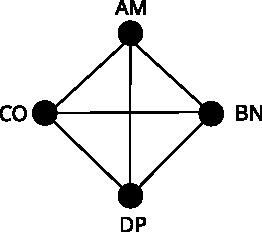
\includegraphics[width=\linewidth]{4clique}
        \end{column}
        \end{columns}
    \end{exampleblock}

    \pause
    \begin{block}{}
        \alert{Can we generalize to uncertain, multidimensional sets of attributes?}
    \end{block}
    
\end{frame}

\section{\PresQ}


%\subsection{Background}

\begin{frame}{Generalization of IND}
    \begin{block}{\alert{Equally-Distributed Dependency (EDD)}}
        \smallskip
        An equally-distributed dependency between a set of columns X
        of relation R and a set of columns Y of relation S, written $R.X \eqdist S.Y$ or
        $X \eqdist Y$, asserts that the values of X and Y follow the same probability distribution.
    \end{block}
\end{frame}

\begin{frame}{Inference Rules}
    \metroset{block=fill}
    \begin{block}{Reflexivity}
        $R[X] \eqdist R[X]$
    \end{block}
    \begin{block}{Transitivity}
        $ R[X] \eqdist S[Y] \land S[Y] \eqdist T[Z] \implies R[X] \eqdist T[Z]$
    \end{block}
    \begin{block}{Permutation and \alert{Projection}}
        If $R[A_1,\dots,A_n] \eqdist S[B_1,\dots,B_n]$ then
        $R[A_{i_1},\dots,A_{i_m}] \eqdist S[B_{i_1},\dots,B_{i_m}]$ for each sequence
        $i_1,\dots,i_m$ of distinct integers from $\{1,\dots,n\}$
    \end{block}
    
    Reflexivity, permutation, and transitivity rules hold
    for $\eqdist$ \footcite{randles1979introduction}.

    For the projection, see \alert{Section 5.1, Proof 1} (page 53).
\note{
    The contribution is the proof of Projection for $\eqdist$.
}
\end{frame}

\begin{frame}{Search Space}
    \metroset{block=fill}
    \begin{block}{Partial Order}
        Let $I_1 = R[X] \eqdist S[Y]$ and $I_2 = R'[X'] \eqdist S'[Y']$.
        
        $I_1$ \textbf{specializes} $I_2$ (denoted $I_1 \prec I_2)$ iff
        \begin{enumerate}
            \item $R = R'$ and $S = S'$.
            \item $X$ and $Y$ are sub-sequences of $X'$ and $Y'$, respectively.
        \end{enumerate}
    \end{block}

\note{
    Partial Order is the same, replacing $\subseteq$ with $\eqdist$,
    which we can do thanks to the previous proofs.
}
\end{frame}

\begin{frame}{Search Space}
    \metroset{block=fill}
    \begin{alertblock}{Satisfiability}
    Let $I = R[X] \eqdist S[Y]$.
    A dataset $d$ \emph{satisfies} $I$ iff  a statistical test fails to reject $H_0: P(R[X]) = P(S[Y])$
    given a significance level $\alpha$.
    This is denoted as $d \models I$.

    \medskip
    
    Given $I_1 \prec I_2$:
    
    \begin{enumerate}
        \item If $d \models I_2$, then $d \models I_1$ (If we can not reject $H_{0_2}$, we can not reject $H_{0_1}$.)
        \item $d \not\models I_1$ with a probability $\alpha$ when $d \models I_2$
            (Rejecting $H_{0_1}$ \emph{does not} imply the rejection of $H_{0_2}$)
    \end{enumerate}
    
    \end{alertblock}

\note{
    \alert{Satisfiability changes}. Purging upwards is not trivial anymore.
    
    \bigskip
    
    ONLY FOR BACKUP
    
    \begin{exampleblock}{Example}
    \smallskip
    If we have two sets of $10$ attributes that are equally distributed, the number of
    3-dimensional projections (specializations) that must be equally distributed will be $\binom{10}{3} = 120$.
    If we have a significance level of $\alpha = 0.1$, the expected number of
    falsely rejected 3-dimensional equalities is $12$.
    \end{exampleblock}
}

\end{frame}

\begin{frame}{Traversal}
    We are using statistical tests.
    
    \begin{itemize}
        \item We may falsely refuse an EDD (type I error)
        \item Or falsely accept it (type II error).
        \item We need to generalize to cliques with missing and spurious edges.
    \end{itemize}
\end{frame}

%\subsection{Quasi-Clique Finding}
\begin{frame}{Quasi-Clique Finding}
    \metroset{block=fill}
    \begin{alertblock}{Definition}
    Given a k-uniform hypergraph $(V,E)$, and two parameters $\lambda, \gamma \in [0,1]$,
    the sub-graph $H'=(V',E')$ induced by a subset $V' \subseteq V$ is a
    $(\lambda-\gamma)$ quasi-clique iff:
    
    \begin{equation}
        |E'| \ge \gamma \cdot \binom{|V'|}{k}
        \label{eq:edge_hyperclique}
    \end{equation}
    
    \begin{equation}
        \forall v \in V': deg_{V'}(v) \ge \lambda \cdot \binom{|V'| - 1}{k - 1}
        \label{eq:deg_hyperclique}
    \end{equation}

    Where $deg_{V'}(v)$ represents the degree of $v$, and $E'$ is a subset of $E$ such that
    $\forall e \in E' : e \subseteq V'$
    \end{alertblock}
    
    We can approximate $\gamma \approx 1 - \alpha$. How do we bound $\lambda$?

\note{
\begin{enumerate}
    \item Constrains the number of missing edges on the quasi-clique wrt the clique
    \item Constrains the number of missing connecting edges for a given node
\end{enumerate}

We can use (1), or (2), or both, which is more resilient.
}
\end{frame}

\begin{frame}{Quasi-Clique Finding}
    \begin{block}{}
    There is no reason to think that any particular subset of the edges
    has a higher probability of having missing members. If a given node has an
    unexpectedly low degree, it is most likely connected by spurious edges.
    \end{block}
    \metroset{block=fill}
    \begin{block}{The degree should follow a hypergeometric distribution}
    \begin{equation}
        \forall v \in V': \operatorname{CDF}(\operatorname{Degree}(v)) \ge \Lambda
    \end{equation}
    \end{block}
    \centering
    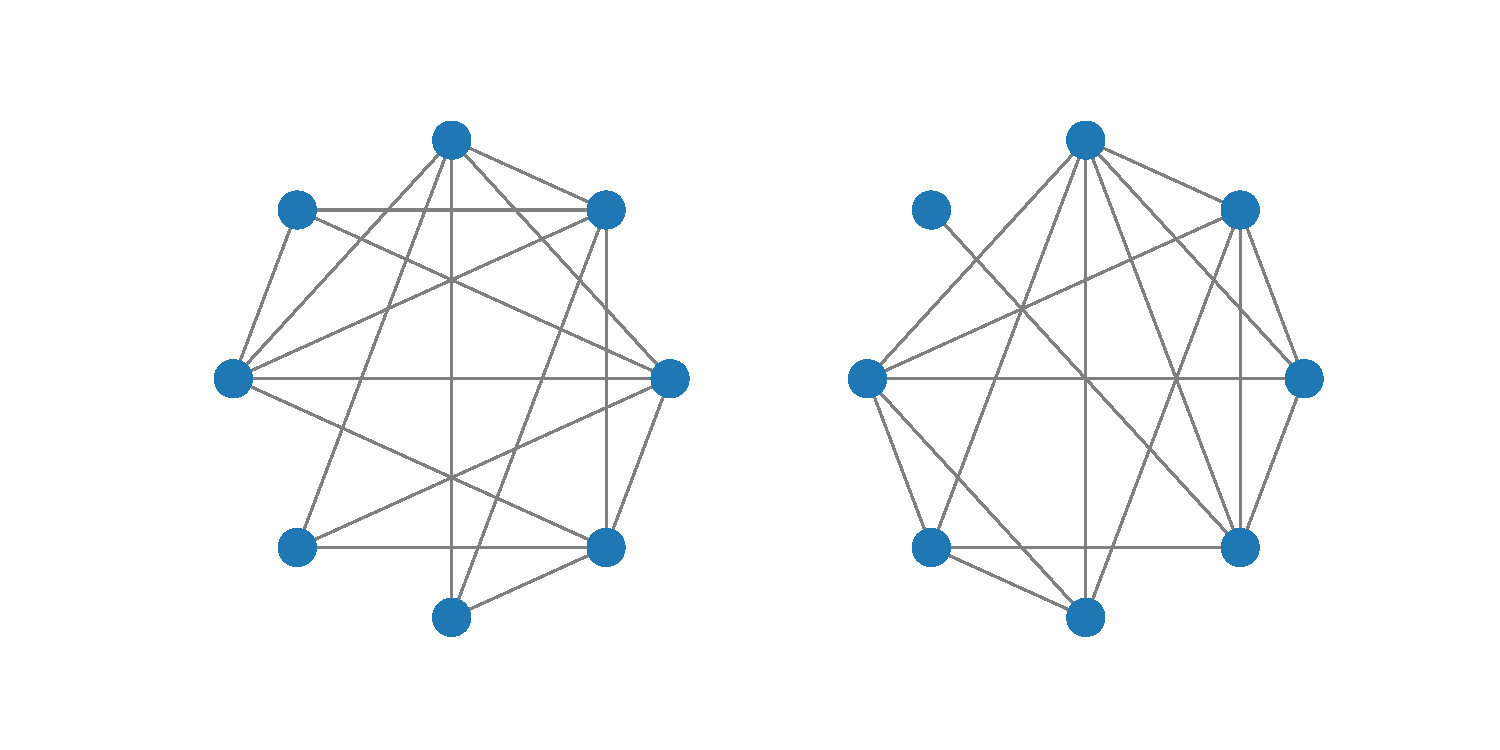
\includegraphics[width=0.6\linewidth]{quasicliques}

\note{
 Hypergeometric: sampling without replacement. Define drawing an edge connecting a node V as a success and any other a failure.
 If the quasi-clique misses |E| edges, and the node has degree(V) missing edges, what's the probability that is just chance?
}
\end{frame}

\begin{frame}{\PresQ}

    \begin{block}{}
    \PresQ is an algorithm for finding quasi-cliques on uniform
    $k$-hypergraphs.
    
    \begin{enumerate}
        \item Finds ``seeds'' using a modified version of \textsc{Hyperclique}~\footcite{koeller2003discovery}.
        \item Grows the ``seeds'' following a tree-shaped, depth-first
        traversal~\footcite{uno_efficient_2010}.
    \end{enumerate}
    \end{block}
    
    \begin{alertblock}{Complexity}
        \smallskip
        The number of maximal cliques is bound by $\Omega(a^{|V|/b})$,
        where $a, b$ are two constants that depend on the rank of the hypergraph.
        
        The worst-case is always going to be exponential.
    \end{alertblock}

\note{
\cite{Tomescu1981} for proof of the number of maximal cliques bound.
}
\end{frame}

%\subsection{Algorithm}

\begin{frame}{}
    \begin{columns}
    \begin{column}{0.5\linewidth}
        \renewcommand{\theenumi}{\alph{enumi}}
        \begin{enumerate}
            \item Generate candidate 1EDD.
            \item If $\eqdist$ can not be rejected, map to nodes.
            \item Test all pairwise combinations (2EDD).
            \item If $\eqdist$ can not be rejected, map to edges on a $k$-hypergraph.
            \item Search for quasi-cliques\label{step:search_quasi}.
            \item Validate quasi-cliques.
            \item Rejected quasi-cliques are used to generate a $k+1$-hypergraph.
            \item Go-to \ref{step:search_quasi}.
        \end{enumerate}
    \end{column}
    \begin{column}{.5\linewidth}
        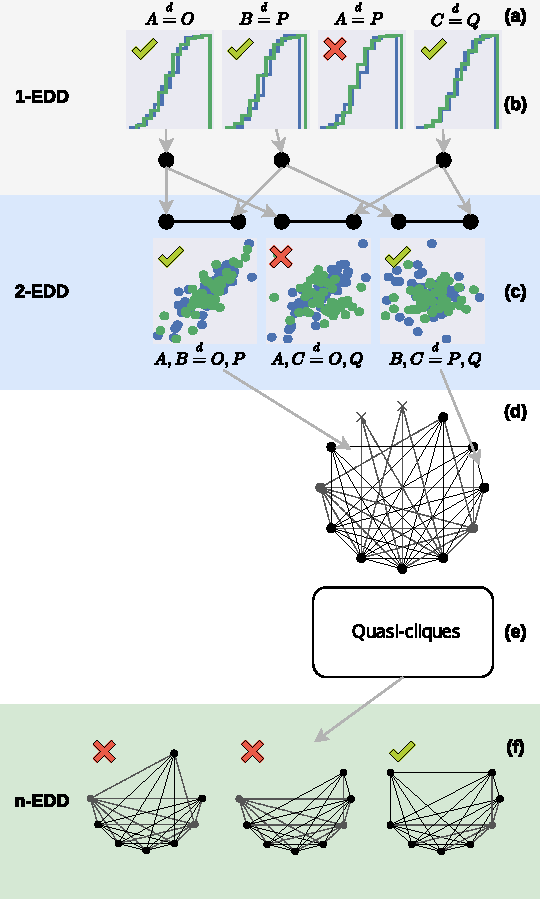
\includegraphics[width=0.9\linewidth]{pipeline}
    \end{column}
    \end{columns}
\end{frame}

\subsection{Evaluation}

\begin{frame}{Clique Recovery: Missing Edges}
    \begin{figure}
        \centering
        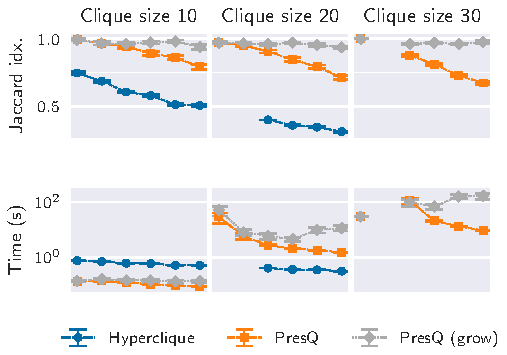
\includegraphics{3hyper_alpha}
        \caption{Robustness wrt. missing edges (3-hypergraph)}
    \end{figure}
\end{frame}

\begin{frame}{Clique Recovery: Correlated Missing / Spurious}
\begin{figure}
    \centering
    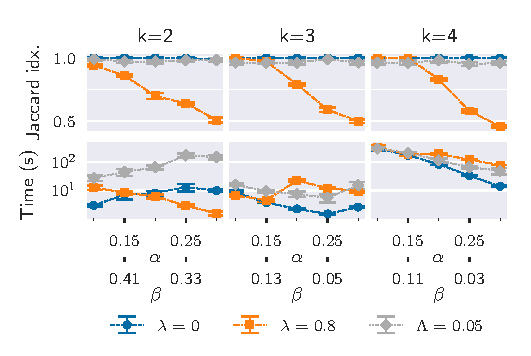
\includegraphics{quasi_corr_20}
    \caption{
    Recovery ratio and run-times for cliques of size 20 on uniform $(2,3,4)$-hypergraphs.
    }
\end{figure}

\note{
Removed and added purely random. With actual data, $\Lambda$ is more robust (next slide).
}
\end{frame}

\begin{frame}{EDD Finding}

\begin{table}
\begin{tabular}{lrrr}
                   & \thead{Quasicliques} & \thead{Valid} & \thead{Median size} \\
$\Lambda = 0.00$   & 2385                 & 292       & 19        \\
$\Lambda = 0.05$   & 107                  & 64        & 12        \\
$\Lambda = 1.00$\footnotemark & \numprint{53 053} & \numprint{52 291} &  6         \\
\end{tabular}
\caption{Consequences of the different $\Lambda$ parameterization when running over the DC2 dataset.}
\end{table}

\begin{block}{}
EDD finding based on quasi-cliques constrained by $\gamma$ and $\Lambda$ 
strike a good balance between the completeness of the result ($7 - 25\%$ on the max. EDD size) and the run time.
\end{block}

\note{
\begin{itemize}
    \item For $\Lambda = 0$, the search algorithm is too greedy and accepts quasi-cliques that are poor candidates.
    Too many are invalid (8 times more candidates than valid) and must be fed back to the algorithm, increasing run-time.
    
    \item For $\Lambda = 1$, the search algorithm is too restrictive. Its precision is high,
     but it spends a long time enumerating small cliques.

    \item $\Lambda = 0.05$ provides the right balance, improving the result and performance.
\end{itemize}

Tables 5.6 and 5.7 contain more detailed results of this experiment.
}
\end{frame}

\begin{frame}{Insights Only From the Data}
\begin{figure}
    \centering
    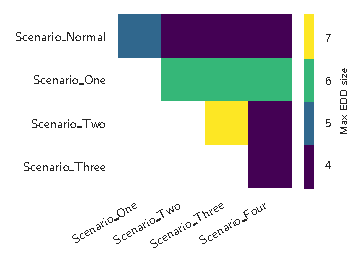
\includegraphics[width=.6\textwidth]{aircraft-cross}
    \caption{
        Without knowing the structure or content of the files from the \emph{Aircraft Fuel Distribution System}
        dataset, we can see that scenarios two and three are the most similar. We can confirm this in
        \cite{Gheraibia2019}.
    }
\end{figure}
\end{frame}

\section{Two-Sample Test Based on Self-Organizing Maps}

%\subsection{Background}

\begin{frame}{Classifier 2-Sample Tests}
    \begin{block}{}
        A binary classifier can be seen as a two-sample test.
        If a classifier has a better-than-chance performance (50\%), the two classes do not originate from the same
        population~\footcite{friedman2004multivariate}.
        \smallskip
        Given two samples $P$ and $Q$:
        \begin{enumerate}
            \item Label samples originating from $P$ with $1$, and those originating from $Q$ with $-1$.
            \item Pool both samples into a single set $U$
        \end{enumerate}
    \end{block}
\end{frame}

\begin{frame}{Classifier 2-Sample Tests}
    \metroset{block=fill}
    \begin{block}{Approach 1~\footcite{friedman2004multivariate}}
        A classifier is trained on $U$ to predict the label. The classifier score function $F(u)$ is used
        to reduce the n-dimensional statistical test to a 1-dimensional statistical test.
    \end{block}
    \begin{block}{Approach 2~\footcite{lopez2016revisiting}}
        $U$ is split into training and test sets. The accuracy of the classifier on the test set is the test statistic.
    \end{block}

\note{
\begin{enumerate}
    \item Approach 1
    \begin{itemize}
        \item $F(u)$ is evaluated on all samples. and we can have two CDF (integrating over $F$), one for P and one for Q. Use unidimensional test.
    \end{itemize}

    \item Approach 2
    \begin{itemize}
        \item Can not use the full set to do the test (a problem for small samples)
        \item Underpowered since it uses a discrete test statistic
    \end{itemize}
\end{enumerate}
}
\end{frame}

\begin{frame}{Self-Organizing Maps}
    An \emph{unsupervised} machine-learning algorithm that learns
    a projection from a high-dimension input space into a low-dimension output space.

    \smallskip
    
    The output space is modeled as a grid of \emph{neurons} that \emph{responds} to a set of
    values from the input space~\footcite{kohonen1982self}.

    \smallskip
    
    \alert{The output model preserves the topology of the input space}: any continuous changes
    in the input data cause a continuous change on the neural map~\footcite{Villmann1999}.
    
    \metroset{block=fill}
    \begin{alertblock}{Insight}
        \smallskip
        If two samples are equally distributed on the input space, they must be equally distributed on the output space.
    \end{alertblock}    

\note{
Thanks to emergent properties, a classifier can be trained on the output space.
}
\end{frame}

%\subsection{Algorithm}

\begin{frame}{SOM 2-Sample Test}
    \begin{block}{Algorithm}
        \begin{enumerate}
        \item Train a SOM $M$ of size $(w, h)$ over $U = X \cup Z$.
        \item Project $X$ and $Z$ separately over the SOM  $M$.
        \item For each neuron $n_i$, count how many points from $X$ ($R_i)$ and how many from $Z$ ($S_i)$ are mapped to it.
        \item Perform a $\chi^2$ two-sample test.
        \end{enumerate}

        Under the null hypothesis, the test statistic follows a $\chi^2$ distribution with $k - c$ degrees of freedom,
        \begin{itemize}
            \item $k$ is the number of cells (neurons) where ${R_i + S_i > 0}$
            \item $c = 1$ if the sample sizes are equal, or $c = 0$ otherwise~\footcite{press1993numerical}.
        \end{itemize}        
    \end{block}
\end{frame}

\begin{frame}{Advantages}
    \begin{itemize}
        \item After the test, we have a trained model that can be used for
            
            \begin{itemize}
                \item Visualization
                \item Clustering~\footcite{ultsch2005esom}
            \end{itemize}

        \item The full dataset is used.
        \item It works with unbalanced sample sizes from $X$ and $Z$.
        \item It can be generalized to non-vectorial data~\footcite{kohonen1982self}.
    \end{itemize}

\note{
Non-vectorial as long as there is a distance metric and training is done in batches
}
\end{frame}

\subsection{Evaluation}

\begin{frame}{Experiment: Multidimensional Normal Distribution}
    \begin{block}{Evaluated Alternatives}
        \smallskip
        \begin{itemize}
            \item Nearest neighbor type coincidences~\footcite{Henze1988, Schilling1986b}.
            \item Classifier two-sample tests.
        \end{itemize}
    \end{block}
    \begin{block}{``Fair'' Distributions}
        \smallskip
        \cite{ramdas2015decreasing} argue that a ``fair'' evaluation of the
        statistical power as the dimensionality increases must keep the
        amount of information fixed.
    \end{block}

\note{
For the location test, fairness can be achieved by two multivariate Gaussians that only differ on the first dimension.
}
\end{frame}

\begin{frame}{}
\begin{figure}
    \centering
    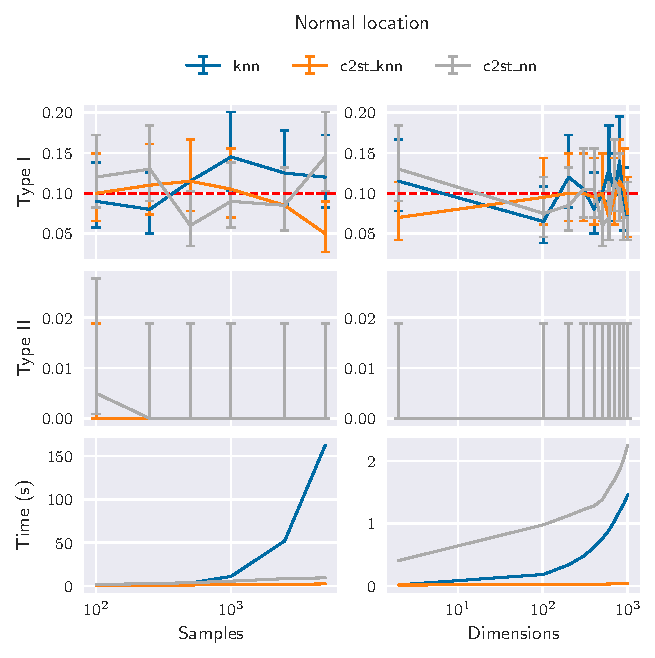
\includegraphics[height=\textheight]{normal_location}
\end{figure}

\note{
    \begin{itemize}
        \item Red-line significance level ($\alpha$) which is fixed
        \item The plot shows an empirical significance level (95\%)
        \item Except for c2st-nn at samples 100, the bars overlap for Type II error.
    \end{itemize}
    DO NOT SAY, BACKUP:
    \begin{itemize}
        \item For the varying number of samples, dimensionality is fixed at 1000 (max)
        \item For the varying number of dimensions, the number of samples is fixed at 300
        \item Repeated 500 times for each data point
    \end{itemize}
}
\end{frame}

\begin{frame}{}
\begin{figure}
    \centering
    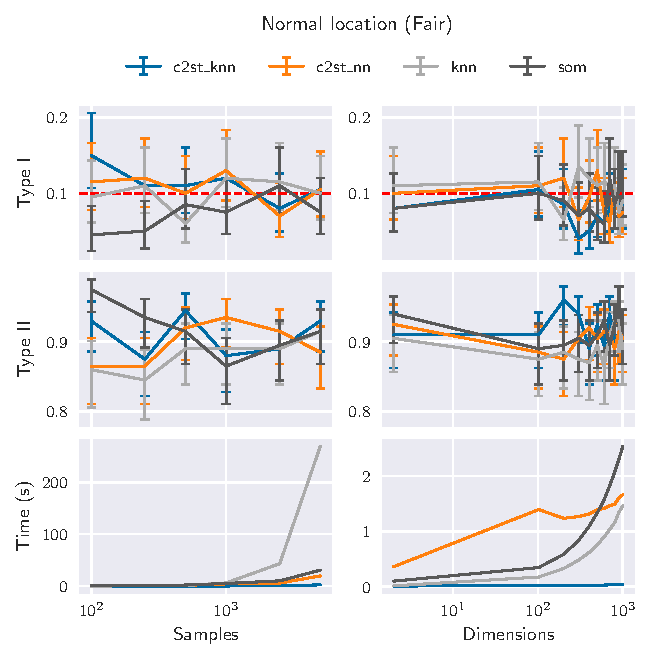
\includegraphics[height=\textheight]{normal_location_fair}
\end{figure}
\end{frame}

\begin{frame}{Experiment: Eye Movement Dataset}
    \begin{block}{Dataset}
        \smallskip
        11 subjects were shown a question and a list of ten 
        sentences: one correct answer (C), four relevant (R), and five irrelevant (I).
        
        Their eye movement was measured for each answer and summarized into 22 features~\footcite{salojarvi2005inferring}.
    \end{block}
    \begin{block}{Evaluated Alternatives}
        \smallskip
        \begin{itemize}
            \item Nearest neighbor type coincidences.
            \item Classifier two-sample tests.
            \item Kernel-Based methods MMD-B~\footcite{zaremba2013b} and Song's~\footcite{song2021fast}.
        \end{itemize}
    \end{block}
\end{frame}

\begin{frame}{}
\begin{table}[htbp]
    \centering
    \begin{tabular}{c r r r r r r}
        \hline
        \multicolumn{7}{c}{\thead{I vs. C}} \\
        \hline
        \thead{m = n} & \thead{Song} & \thead{MMD-B} & \thead{KNN} & \thead{C2ST-KNN} & \thead{C2ST-NN} & \thead{SOM} \\
        \hline
        100 & 0.826 & 0.374 & \textbf{0.973} & 0.164 & 0.079 & 0.042 \\
        200 & 0.998 & 0.850 & \textbf{1.000} & 0.565 & 0.349 & 0.947 \\
        300 & \textbf{1.000} & 0.985 & \textbf{1.000} & 0.863 & 0.644 & \textbf{1.000} \\
        400 & \textbf{1.000} & \textbf{1.000} & \textbf{1.000} & 0.968 & 0.882 & \textbf{1.000} \\
        \\
        \hline
        \multicolumn{7}{c}{\thead{R vs. C}} \\
        \hline
        \thead{m = n} & \thead{Song} & \thead{MMD-B} & \thead{KNN} & \thead{C2ST-KNN} & \thead{C2ST-NN} & \thead{SOM} \\
        \hline
        100 & 0.670 & 0.236 & \textbf{0.845} & 0.062 & 0.023 & 0.007 \\
        200 & 0.969 & 0.685 & \textbf{0.996} & 0.298 & 0.139 & 0.672 \\
        300 & 0.999 & 0.941 & \textbf{1.000} & 0.558 & 0.314 & 0.987 \\
        400 & \textbf{1.000} & 0.988 & \textbf{1.000} & 0.811 & 0.560 & \textbf{1.000} \\
    \end{tabular}
    \caption{Empirical statistical power for the eye movement datasets.}
    \label{tab:eye}
\end{table}
\end{frame}

\begin{frame}{Interpretability}
    \begin{figure}
        \centering
        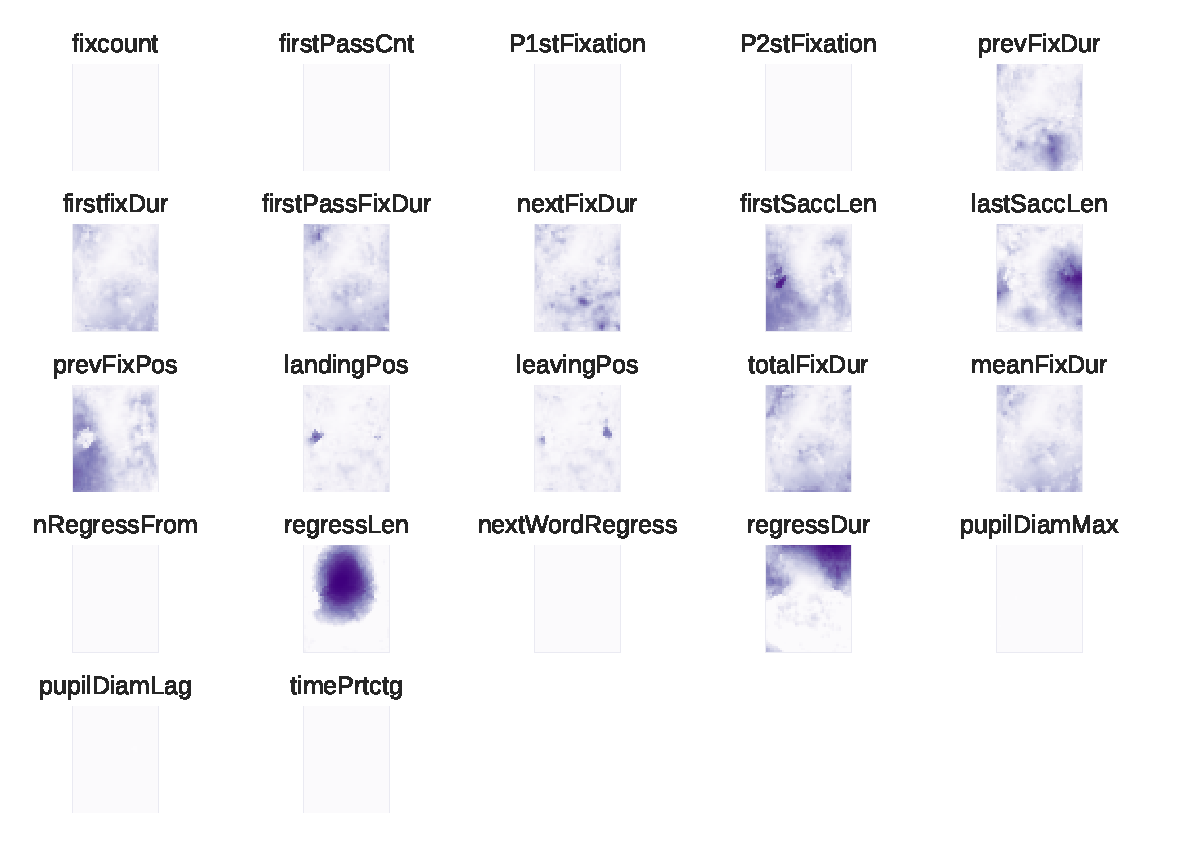
\includegraphics[trim=5pt 75pt 5pt 5pt,clip,width=0.9\textwidth]{eye_features.eps}
        \caption{
            The features ``Regression length'' and ``regression duration'' stand out,
            which is expected to happen when reading a correct answer.
        }
    \end{figure}
\note{
\begin{itemize}
    \item Regression length and duration are related to re-reading a word.
    \item \cite{salojarvi2005inferring}
    \item Codebooks for a subset of the parameters: how each neuron is sensitive to a given feature. Darker is more.
\end{itemize}
}
\end{frame}


\begin{frame}{Caveat}
    \begin{itemize}
        \item \cite{rosenblatt2019better} argue that provable test statistics
            should be preferred over heuristic alternatives.
        \item This proposal is oriented toward exploring abundant structured data.
        \item Developing a tailored statistic for all possible combinations is not viable,
            and a pragmatic approach is more suitable~\footcite{kim2021classification}.
    \end{itemize}
\end{frame}

\section{Threats to Validity}

\begin{frame}{Internal Validity}
    \begin{alertblock}{Significance of the Results}
        \smallskip
        The presented results could be a statistical fluctuation. To reduce the risk:
        
        \begin{itemize}
            \item The tests have been randomized and measured multiple times.
            \item The uncertainties are explicitly reported using either 95\% confidence intervals or quartiles.
        \end{itemize}
    \end{alertblock}
\end{frame}

\begin{frame}{Internal Validity}
    \begin{alertblock}{Implementation Bias}
        \smallskip
        The evaluated \PresQ and \textsc{Find} implementations share most parts of the code. The differences can only originate
        from the algorithms and not the implementations.
        
        \smallskip
        
        For the statistical tests, SOM, $k$NN, C2ST-NN and C2ST-kNN have all been implemented using well known
        Python libraries (\textsc{somoclu}, \textsc{numpy}, \textsc{scikit-learn}).
    \end{alertblock}
\end{frame}

\begin{frame}{External Validity}
    \begin{alertblock}{Generalization of the results}
        \smallskip
        The tests were performed with a multitude of datasets from different domains.
        
        \smallskip

        In the interests of transparency, the SOM statistical test has been tested on a set
        of ``fair'' distributions explicitly designed to show the shortcomings of multidimensional statistical tests.
        
    \end{alertblock}
\end{frame}

\section{Future Work \& Conclusion}

\begin{frame}{Future Work}
    \begin{block}{Performance improvements}
        \begin{itemize}
            \item Improve the quasi-clique finding algorithm.
            \item Data-aware quasi-clique finding algorithms.
            \item Dimensionality reduction before EDD finding.
        \end{itemize}
    \end{block}

    \begin{block}{Generalization}
        \begin{itemize}
            \item \alert{Partial equality-of-distribution}
            \item Bayesian EDD finding algorithms.
            \item \alert{Multidimensional \emph{complementarity}}
        \end{itemize}
    \end{block}

    \begin{block}{Applications}
        \begin{itemize}
           \item Applications on privacy-preserving data mining.
        \end{itemize}    
    \end{block}
   

\note{
\begin{itemize}
    \item Data-aware: Somehow, considering correlation matrix, for instance?
    
    \item Bayesian: can check local null hypothesis testing so that we can accept a candidate with only partial support.
         Support for priors~\footcite{soriano2015bayesian}.
    \item Multidimensional \emph{complementarity} (i.e., a dataset may be split 
          based on the values from a given set of attributes).
          
    \item Privacy-preserving: linking attacks
    \begin{itemize}
        \item  Experiment with Open University Learning Analytics Dataset shows an "attribute disclosure": the attackers improve their knowledge of a set of attributes for a given individual. i.e., young females from North Western, most likely deprived (low income, low employment, etc.).
    \end{itemize}
\end{itemize}
}
\end{frame}

\begin{frame}{Contributions}

\begin{alertblock}{\emoji{check-mark} Find existing techniques that help users to explore the data in situ}
    \begin{itemize}
        \item Survey of the State of the Art
    \end{itemize}
\end{alertblock}

\begin{alertblock}{\emoji{check-mark} Identify gaps in the coverage of the existing techniques}
    \begin{itemize}
        \item New category for IDE: \alert{Schema Homogenization}
        \item Equally-Distributed Dependency
    \end{itemize}
\end{alertblock}

\begin{alertblock}{\emoji{check-mark} Design new algorithms tailored to numerical and uncertain data}
    \begin{itemize}
        \item \PresQ
        \item Two-Sample Test Based on SOM
    \end{itemize}
\end{alertblock}

\end{frame}

\begin{frame}{Conclusion}

\metroset{block=fill}
\begin{block}{\emoji{white-check-mark} Main Objective}
    The proposed algorithms can assist data scientists in identifying relationships
    between numerical, raw datasets distributed across multiple files
    based solely on their intrinsic distribution.
\end{block}

\end{frame}

\appendix

\definecolor{myblue}{RGB}{35,55,59}
{\setbeamercolor{palette primary}{fg=white, bg=myblue}
\begin{frame}[standout]
  \huge Questions?
\end{frame}
}

{\setbeamercolor{palette primary}{fg=black, bg=black!2}
\begin{frame}{}
  \begin{minipage}[b][\paperheight]{\textwidth}
    \usebeamertemplate*{title graphic}
    \vfill
    \usebeamertemplate*{title}
    \usebeamertemplate*{title separator}
    \usebeamertemplate*{author}
    \usebeamertemplate*{date}
    \usebeamertemplate*{institute}
    \vspace{4em}
    \begin{center}
        \raisebox{-0.5\height}{
\includegraphics[width=4em]{CC_BY_icon}}
        \hspace{2em}
        \raisebox{-0.6\height}{
\includegraphics[width=4em]{MIT}}
        \hspace{2em}
        \raisebox{-0.5\height}{
\includegraphics[width=4em]{zenodo}}
    \end{center}
    \begin{center}
        \footnotesize
        \href{https://doi.org/10.5281/zenodo.6865856}{10.5281/zenodo.6865856}
        \hspace{2em}
        \href{https://doi.org/10.5281/zenodo.7452720}{10.5281/zenodo.7452720}
    \end{center}
    \vfill
    \vspace*{1mm}
\end{minipage}
\end{frame}
}

{\setbeamercolor{palette primary}{fg=white, bg=black}
\begin{frame}[standout]
  Backup slides
\end{frame}
}

\begin{frame}{Proof of Projection}
\small
We need to prove that if two sets of random variables
$X_1,\dots,X_n$ and $Y_1,\dots,Y_n$ are equally distributed, so are
any of their possible sub-sequences.

Let $X'$ and $Y'$ be the sequences $X_1,\dots,X_m$ and $Y_1,\dots,Y_m$ with $m < n$.
Their corresponding  CDF are just the \emph{marginal} CDF:

\begin{equation}
\begin{split}
    F_{X_1,\dots,X_m}(x_1,\dots,x_m) = & F_{X_1,\dots,X_m,X_{m+1},X_n}(x_1,\dots,x_m,x_{m+1},\dots,x_n) \\
    F_{Y_1,\dots,Y_m}(y_1,\dots,y_m) =& F_{Y_1,\dots,Y_m,Y_{m+1},Y_n}(x_1,\dots,x_m,x_{m+1},\dots,x_n)\\
    & \forall (x_1,\dots,x_m) \in \mathbb{R}^m \textrm{ and } x_i \xrightarrow{} \infty \; \forall i > m
\end{split}
\end{equation}

Since $X_1,\ldots,X_n \eqdist X_1,\ldots,Y_n$, the right-hand side of both equations must be the same.
By transitivity, 

\begin{equation}
\begin{split}
    & F_{X_1,\dots,X_m}(x_1,\dots,x_m) = F_{Y_1,\dots,Y_m}(y_1,\dots,y_m) \; \forall (x_1,\dots,x_m) \in \mathbb{R}^m \\
    & \implies X_1,\dots,X_m \eqdist Y_1,\dots,Y_m
\end{split}
\end{equation}

\note{
Since $F$ is the CDF, it is the integral of the probability function at that point.

$F_X(x) = \lim_{y \to \infty} F(x,y)$
}

\end{frame}

\begin{frame}{Pairwise matching is not sufficient}
\begin{figure}
    \centering
    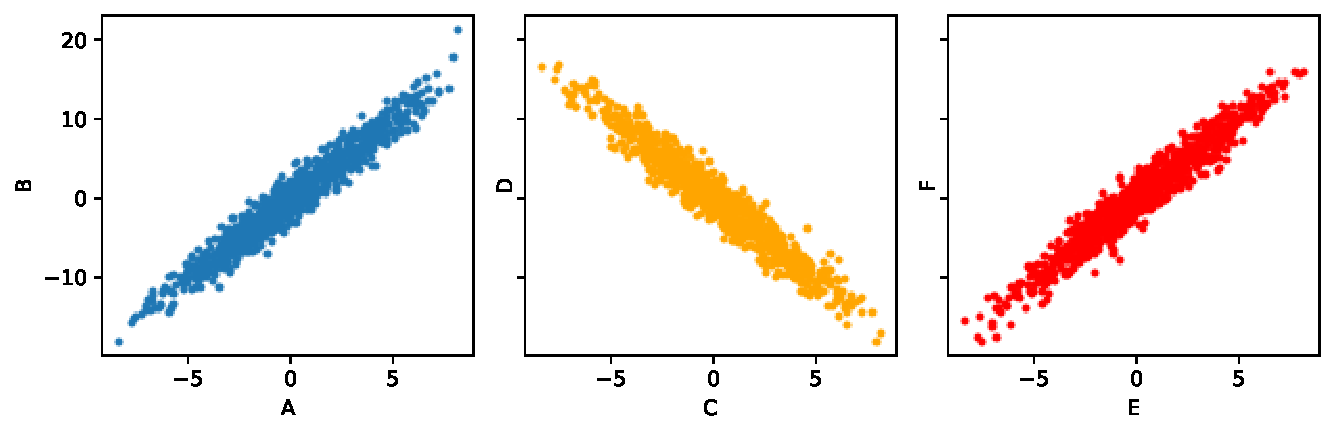
\includegraphics[width=\textwidth]{no2ind.pdf}
    \caption{Example of a 2D distribution where the pairwise matching is insufficient}
\end{figure}
\end{frame}

\begin{frame}{Clique Recovery: Spurious Edges}
    \begin{figure}
        \centering
        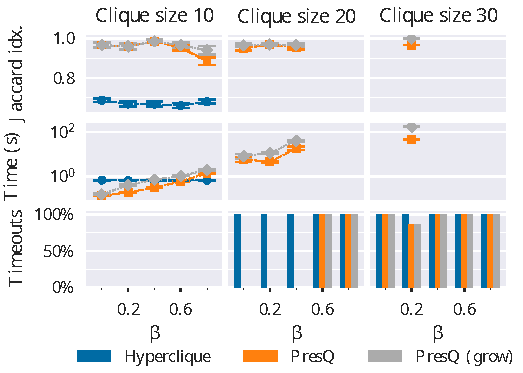
\includegraphics{3hyper_beta}
        \caption{Robustness wrt. spurious edges (3-hypergraph)}
    \end{figure}
\end{frame}

\begin{frame}{PresQ Scalability}
\begin{figure}
    \centering
    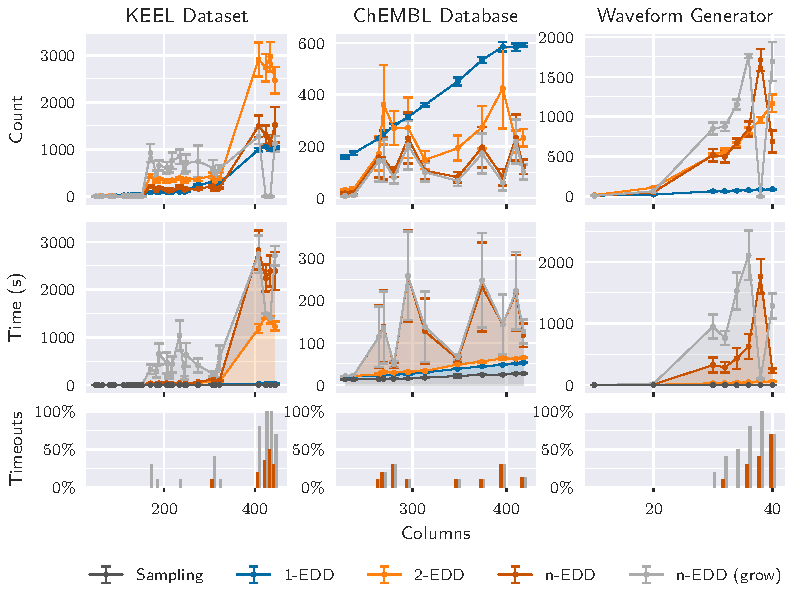
\includegraphics[width=\textwidth]{scalability.pdf}
\end{figure}
\end{frame}

\begin{frame}{PresQ Scalability}
\begin{figure}
    \centering
    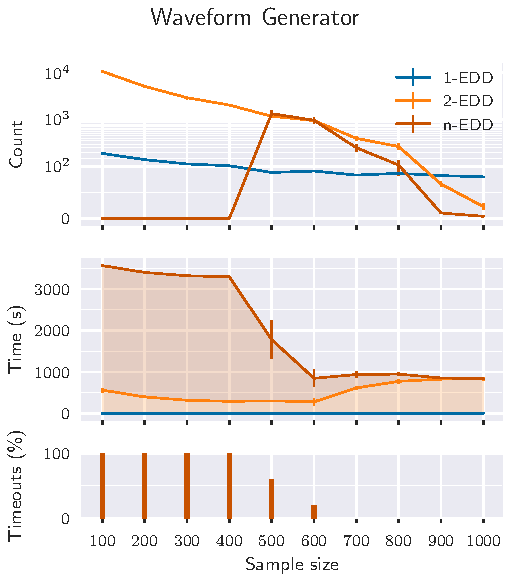
\includegraphics[height=\textheight]{scalability_sample_wave.pdf}
\end{figure}
\end{frame}

\begin{frame}{Eye Regress}
\begin{figure}
    \centering
    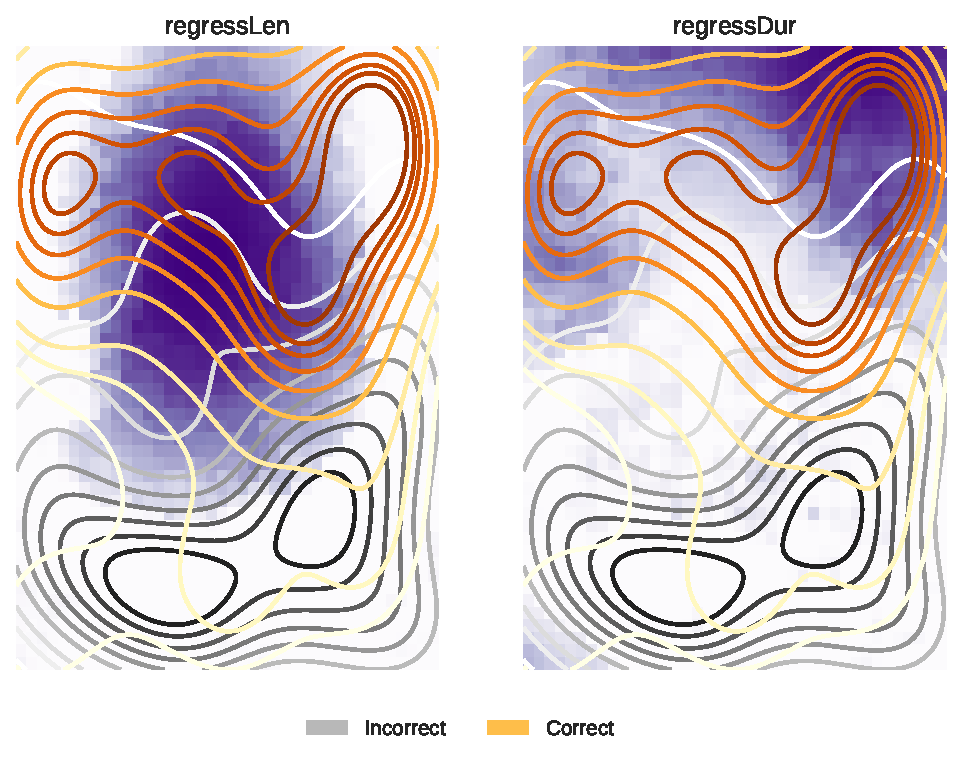
\includegraphics[height=\textheight]{eye_regress-eps-converted-to.pdf}
\end{figure}
\end{frame}

\begin{frame}{Open University Learning Analytics Dataset}
\begin{figure}[t]
    \centering
    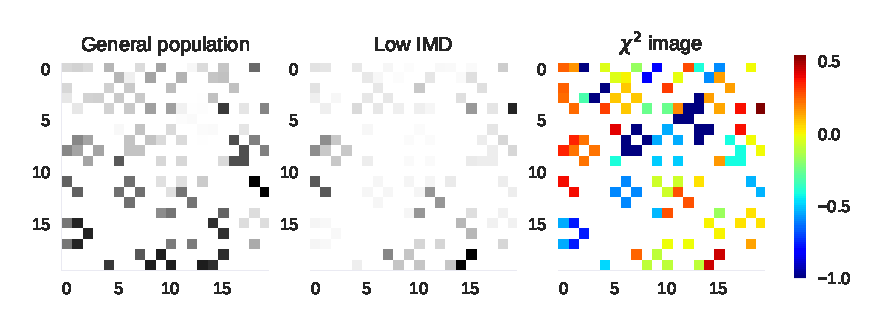
\includegraphics[width=\textwidth]{imd}
    \caption[Comparing \glsfmtlong{SOM} density variations.]{Density of samples for the general population (left), poorest segment (center) and
    relative difference (right). Cells with a value of $-1$ do not have any low-income students,
    while those with a value of $0.5$ show an ``excess'' with respect to the general
    population.}
\end{figure}
    \cite{kuzilek_open_2017}
\note{
Let us consider the case of a researcher with the hypothesis that gender, age, and
region of origin influence a student's economic situation, or perhaps they could
be trying to deanonymize the data.
}
\end{frame}

\begin{frame}{Open University Learning Analytics Dataset}
\begin{figure}[htbp]
    \centering
    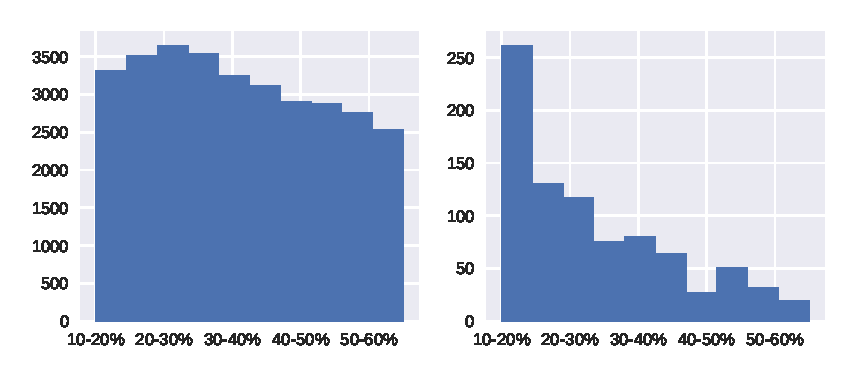
\includegraphics[width=0.8\textwidth]{imd_histogram}
    \caption[Histogram of the \glsfmtlong{IMD} for two populations.]{
        \emph{Indices of Multiple Deprivations} for the general population (left) and for
        young female students from the \emph{North Western Region}.
    }
    \begin{block}{}
    One of the cells with the highest bias toward low-income students
    contains only young female students from the \emph{North Western Region}.
    The income for this demographic is skewed toward the low end.
    \end{block}
\end{figure}
\note{
We could obtain this hindsight without prior knowledge of which
attributes correlate with the difference, only with the ``hunch'' that
there is a relation. Thus, we prove that our proposed test can be useful for data exploration.
}
\end{frame}

\end{document}
